% DRAFT - numbers from results/final_tables.md (regenerate with syn/final_tables.py).
% IEEE Computer Society conference format (as required by ARITH: <= 8 pages
% including references, double-blind - anonymise the author block and the
% repository URL in the submitted version).
\documentclass[conference,compsoc]{IEEEtran}
\ifCLASSOPTIONcompsoc
  \usepackage[nocompress]{cite}
\else
  \usepackage{cite}
\fi
\usepackage{amsmath,amssymb}
\usepackage{graphicx}
\usepackage{booktabs}
\usepackage{siunitx}
\usepackage{url}

\begin{document}

\title{The Cost of Exactness in Microscaling Dot Products:\\
An Open, Bit-Accurate Study Across All OCP MX Formats}

% main_anon.tex defines \ANON and \input{}s this file for double-blind review.
\ifdefined\ANON
\author{\IEEEauthorblockN{Anonymous Author(s)}
\IEEEauthorblockA{Submission under double-blind review}}
\else
\author{\IEEEauthorblockN{Oussama Riahi}
\IEEEauthorblockA{Independent Researcher\\ oussmahdi00@gmail.com}}
\fi

\maketitle

\begin{abstract}
Dot-product units for the OCP Microscaling (MX) formats must decide how
precisely to sum the block products before adding the FP32 accumulator.
Published designs make this choice once and justify it in isolation: some
sum exactly and round once, others align every term to the largest exponent
and truncate to a fixed window.  We compare the two policies on equal terms
for all six MX element formats.  A single parameterised open-source RTL code
base implements both, each verified bit-for-bit in cocotb against an exact
rational reference, and both go through the same Yosys/OpenROAD flow on ASAP7
and sky130, with energy from gate-level simulation of the placed netlists.
The cost of exactness is set by each format's exponent range, and the
crossover is sharp: for MXFP4, MXFP6 and MXINT8 the exact unit is 21--47\%
smaller, uses 12--32\% less energy and, except for MXINT8, is 7--9\% faster
than a 24-bit truncating unit, while MXFP8 E4M3 is roughly break-even and
only MXFP8 E5M2 pays clearly (+85--96\% area, +19--28\% energy).  Truncation
at 24 bits is accurate enough in GEMM-style accumulation for the
floating-point formats, but not for MXINT8 on data with outliers, where it
raises the 99th-percentile relative error by about $4000\times$.  Exact
accumulation should therefore be the default for every MX format except
E5M2.  All RTL, models, scripts and data are open source.
\end{abstract}

\section{Introduction}
Low-precision block formats have become the default for machine-learning
arithmetic.  The OCP Microscaling (MX) specification~\cite{ocp_mx}
standardises six element formats (MXFP8 E4M3 and E5M2, MXFP6 E3M2 and E2M3,
MXFP4 E2M1, MXINT8) that share one E8M0 power-of-two scale per block of
$K=32$ elements.  The core operation is the scaled block dot product with
FP32 accumulation,
\begin{equation}
  r = \mathrm{rnd}_{32}\Bigl(c + 2^{x_a-127}\,2^{x_b-127}\sum_{i<K} a_i b_i\Bigr),
  \label{eq:dot}
\end{equation}
whose internal precision the specification leaves to the implementer.

Two policies dominate.  \emph{Exact} units place every product on a common
fixed-point grid, sum without loss and round once~\cite{lutz2024fp8,desrentes2023exact}.
\emph{Anchored truncation} aligns all terms to the largest exponent and keeps
a fixed window of $W$ bits, as in many-term dot-product units for machine
learning~\cite{kaul2019dot,hickmann2020nnpt} and, per microbenchmarking,
in GPU tensor cores up to the MX-capable Blackwell
generation~\cite{fasi2021tensor,khattak2025tensor,rout2025tenfour}.  A third line of
work reduces the accumulator precision further~\cite{cuyckens2025mx}.  Each
design justifies its choice in its own context, with different formats,
technologies and tools.  What is missing is a like-for-like measurement of
what exactness costs, and what truncation loses, format by format.

This paper provides that measurement.  Our contributions:
\begin{itemize}
  \item One open, parameterised RTL code base with exact and anchored-truncation
        datapaths sharing decoders, pipeline cuts and final rounding, for
        all six MX formats, mixed pairs and any power-of-two $K$
        (Section~\ref{sec:arch}).
  \item A verification stack in which every policy has a bit-accurate model,
        the models are checked against an exact rational reference, and the
        RTL is checked bit-for-bit against the models in cocotb
        (Section~\ref{sec:verif}).
  \item Error measurements against the exact reference for single blocks and
        4096-long accumulations, on Gaussian, heavy-tailed and outlier data
        (Section~\ref{sec:accuracy}).
  \item Area, delay and gate-level energy on ASAP7 and sky130 with the
        method stated in full (Sections~\ref{sec:method}--\ref{sec:cost}).
  \item A simple design rule that follows from the data (Section~\ref{sec:disc}).
\end{itemize}

\section{Background and Related Work}
\subsection{MX formats}
Each MX element format is either a small floating-point format or an
8-bit integer with implicit scale $2^{-6}$.  Table~\ref{tab:grid} lists the
properties that matter here: the significand width, and the span of product
exponents, which sets the width of an exact fixed-point grid.  For $K=32$
the exact sum of products needs between 13 bits (E2M1) and 69 bits (E5M2).

\begin{table}[t]
\centering
\caption{Width of the exact fixed-point sum for $K=32$ (magnitude bits)}
\label{tab:grid}
\begin{tabular}{lrrr}
\toprule
Format & significand & product exp.\ span & $|\Sigma|$ width \\
\midrule
MXFP4 E2M1 & 2 & 4  & 13 \\
MXFP6 E2M3 & 4 & 4  & 17 \\
MXFP6 E3M2 & 3 & 12 & 23 \\
MXINT8     & 8 & 0  & 21 \\
MXFP8 E4M3 & 4 & 28 & 41 \\
MXFP8 E5M2 & 3 & 58 & 69 \\
\bottomrule
\end{tabular}
\end{table}

\subsection{Related work}
Lutz et al.~\cite{lutz2024fp8} present two microarchitectures for an exact
FP8 4-way dot product with scaling and FP32 accumulation in 5\,nm; our exact
datapath is close to their late-accumulation design, generalised to all MX
formats and to $K=32$.  Desrentes et al.~\cite{desrentes2023exact} build
exact dot products for 8-bit formats with a fixed-point accumulator.
Kaul et al.~\cite{kaul2019dot} and Hickmann et al.~\cite{hickmann2020nnpt}
describe many-term BF16 units that align to the maximum exponent and truncate
to an internal width, the organisation we use as the truncating baseline.
Among MX-specific designs, MXDOTP~\cite{islamoglu2025mxdotp} adds an MXFP8
dot-product instruction to a RISC-V core, Cuyckens et
al.~\cite{cuyckens2025mx} build precision-scalable datapaths for all six
formats with a deliberately shortened accumulator, Ten-Four~\cite{rout2025tenfour}
is an open fused dot-product unit matching NVIDIA tensor-core truncation, and
Samson et al.~\cite{samson2024fpga} provide open FPGA MX arithmetic.
Closest to our question, Abdurakhmanov and Fahmy~\cite{abdurakhmanov2025mxfpga}
compare exact (Kulisch-style) with BF16 accumulation in MXFP6 and MXFP8
systolic arrays on FPGAs, reporting accuracy, resources and throughput.
Khattak and Mikaitis~\cite{khattak2025tensor} build bit-accurate software
models of NVIDIA tensor cores up to the Blackwell generation; like Fasi et
al.~\cite{fasi2021tensor} they find products aligned to the largest
exponent and truncated to a fixed number of fractional bits, i.e., the
anchored-truncation policy we use as the baseline.
% Khattak & Mikaitis reportedly measure 25 fractional bits for FP8 inputs on
% a Blackwell GPU; confirm the figure in the full text before quoting it.
Islam and Mikaitis~\cite{islam2026mxsim} provide a numerical MX simulator
with configurable accumulator precision but no hardware cost.  Van
Baalen et al.~\cite{vanbaalen2023fp8} argue qualitatively that fixed-point
(Kulisch~\cite{kulisch}) accumulation suits INT8 while floating-point
accumulation suits FP8; Uguen and de Dinechin~\cite{uguen2017kulisch}
explore Kulisch accumulators on FPGAs.  To our knowledge this is the first
comparison of exact and anchored-truncation MX dot products that covers all
six MX element formats on an ASIC flow, with error measured against an exact
reference and energy from gate-level simulation, using one shared,
bit-verified code base for both policies.

\section{Architectures}\label{sec:arch}
Both units implement~\eqref{eq:dot} with a single round-to-nearest-even to
binary32, including subnormal results and overflow to infinity.  They share
the element decoders, the special-value logic (NaN/Inf/signed zero following
IEEE~754 on the exact expression) and the final normalise-and-round stage,
and they differ only in how terms are brought together.  Both accept
\texttt{PIPE[3:0]} to select four optional register cuts; in both the first
cut registers the raw \{product, $e_a+e_b$, sign\} per lane, before any
alignment.

\subsection{Exact unit}
Each product $m_a m_b$ is shifted left by $e_a+e_b$ onto a grid whose LSB is
the smallest product exponent, giving an exact two's-complement term of the
width in Table~\ref{tab:grid}.  A binary adder tree that grows one bit per
level sums the $K$ terms exactly.  The sum $S$ is converted to sign-magnitude,
both $S$ and $c$ are normalised with log-depth leading-zero counters, and the
smaller is right-shifted into a window of $\max(|\Sigma|,24)+3$ bits whose
LSB is a sticky bit.  Because both operands are left-aligned with three zero
bits below, any bit lost to the sticky position implies an alignment
distance of at least four, so an effective subtraction cancels at most one
leading bit and guard, round and sticky are exact (the argument is in the
model's source).  A final LZC, denormalisation for subnormal results and RNE
complete the operation.

\subsection{Truncating unit}
A balanced max tree over the per-lane $e_a+e_b$ of non-zero products, and a
comparison with the exponent of $c$, give the anchor: the largest
\emph{nominal} exponent, taken directly from the operand exponents without
normalising subnormals, as in hardware.  Every term is right-shifted into a
$W$-bit window whose top bit is the anchor, truncating towards zero; the
window is summed by the same adder tree, $c$ is added, and the result goes
through the same normalise-and-round stage.

\section{Verification}\label{sec:verif}
A Python reference computes~\eqref{eq:dot} with exact rationals and rounds
once; its decoders match \texttt{ml\_dtypes} on every code point and its
rounding matches IEEE float64$\to$float32 conversion on 200{,}000 values
including forced ties.  A bit-true model of each datapath uses bounded
integer arithmetic mirroring the RTL widths; the exact model matches the
reference on directed-random vectors for all formats, mixed pairs and
$K\in\{1,2,4,32\}$, and exhaustively for $K=1$ on the FP4/FP6 formats.
Writing this model first exposed a real sizing bug (E5M2 Inf/NaN encodings
overflowing a lane) before any RTL existed.  The cocotb testbench streams
vectors with random valid gaps and compares every output bit-for-bit: 14
configurations of the exact unit and 17 of the truncating unit (all formats,
$W\in[12,40]$, $K\in\{1,8,16,32\}$, pipelined and mixed) pass.  Stimulus is
weighted towards specials, extreme and subnormal elements, cancelling blocks
and a $c$ that nearly cancels the dot product.  Every gate-level power
simulation (Section~\ref{sec:method}) also re-checks the placed netlist
bit-for-bit against the model.

\section{Accuracy of Truncation}\label{sec:accuracy}
Inputs are drawn from $\mathcal{N}(0,1)$, Student-$t$ ($\nu=3$), and a
Gaussian with 1\% of elements scaled by 20--100$\times$ to mimic the outlier
channels of LLM activations, then quantised with the OCP scale rule.  All
data is synthetic.  We measure two things (Table~\ref{tab:acc},
Fig.~\ref{fig:acc}): the share of single-block results that differ from the
exact unit when $c$ has the dot product's magnitude, a stress test for
cancellation, and the 99th-percentile relative error of 4096-long GEMM rows
computed as 128 chained blocks, against the true value of the quantised
inputs.

\begin{figure}[t]
\centering
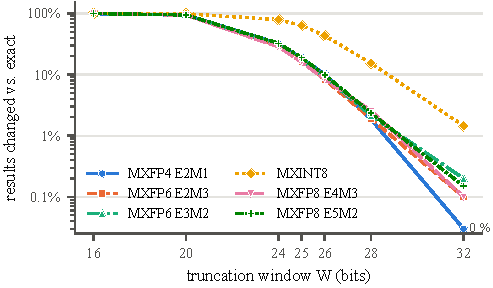
\includegraphics[width=\columnwidth]{figs/accuracy_vs_w.pdf}
\caption{Share of single-block results (Gaussian data, $c$ at the dot
product's magnitude) that anchored truncation changes, versus window width.
The floating-point formats coincide; MXINT8 needs about four more bits.}
\label{fig:acc}
\end{figure}

\begin{table}[t]
\centering
\caption{Accuracy of anchored truncation (synthetic data)}
\label{tab:acc}
\setlength{\tabcolsep}{3pt}
\begin{tabular}{lrrrrr}
\toprule
& \multicolumn{2}{c}{block: \% changed} & \multicolumn{3}{c}{chain, outlier data: p99 rel.\ err.} \\
\cmidrule(lr){2-3}\cmidrule(lr){4-6}
Format & $W{=}24$ & $W{=}32$ & exact & $W{=}24$ & $W{=}28$ \\
\midrule
E2M1 & 31.9 & 0.0 & 0       & 0       & 0 \\
E2M3 & 29.5 & 0.1 & 0       & 0       & 0 \\
E3M2 & 30.4 & 0.2 & 1.8e-7  & 4.0e-7  & 1.8e-7 \\
INT8 & 79.1 & 1.4 & 5.0e-8  & 2.1e-4  & 1.1e-6 \\
E4M3 & 28.4 & 0.1 & 1.3e-6  & 3.6e-6  & 1.3e-6 \\
E5M2 & 32.4 & 0.1 & 1.6e-6  & 1.8e-6  & 1.6e-6 \\
\bottomrule
\end{tabular}
\end{table}

In the stress test, $W=24$ changes about 30\% of results for every
floating-point format and 79\% for MXINT8, whose 8-bit significands produce
16-bit products that a narrow window cuts into.  In realistic accumulation
the picture is milder: for the floating-point formats $W=24$ stays at the
FP32 rounding floor, and on Gaussian data the exact FP4 and FP6 results are
bit-for-bit the true value because the whole sum fits in FP32.  MXINT8 is the exception: with
outliers, $W=24$ raises the 99th-percentile error from $5\times10^{-8}$ to
$2.1\times10^{-4}$, and $W\approx28$ is needed to match exact.

\section{Method for Cost Measurements}\label{sec:method}
Both units go through OpenROAD-flow-scripts~\cite{ajayi2019openroad} with
Yosys synthesis on ASAP7~\cite{clark2016asap7} and sky130hd, with zero I/O
delay so that combinational configurations report input-to-output delay.
\begin{itemize}
  \item \textbf{Area} is standard-cell area after synthesis.  Ratios after
        synthesis matched fully routed ratios within 1\% on ASAP7 (FP4 0.55
        vs 0.54, E4M3 1.18 vs 1.17).  Re-synthesis moved absolute areas by up
        to 3\%.
  \item \textbf{Delay} is the best achieved after clock-tree synthesis (CTS)
        with an aggressive target.
  \item \textbf{Energy} is measured after CTS with the clock target set to
        $1.1\times$ each design's achieved delay, so timing repair does not
        inflate either design.  The placed netlist is simulated in Icarus
        Verilog on 512 MX-quantised Gaussian vectors arranged as GEMM rows
        ($c$ fed back), the VCD is annotated into OpenSTA (100\% of pins
        annotated), and energy is reported per dot product.  Simulation is
        zero-delay, so glitch power is not included.  After-CTS energy was
        within 1\% of fully routed energy on the pipelined FP8 unit, while
        placement-only energy missed the clock network and was 49\% low.
        OpenROAD's vectorless estimate was about $76\times$ too high on this
        arithmetic and is not used.  sky130 cell simulation models were
        generated from the Liberty functions.
\end{itemize}
Unless noted, results are for $K=32$ and single-cycle units, so that no
register placement is involved in the comparison.  An attempt to balance
pipelined versions with ABC retiming produced inconsistent results (the
exact unit became slower; the truncating unit's flip-flops nearly
tripled) and is not used.

\section{Cost of Exactness}\label{sec:cost}

\begin{figure}[t]
\centering
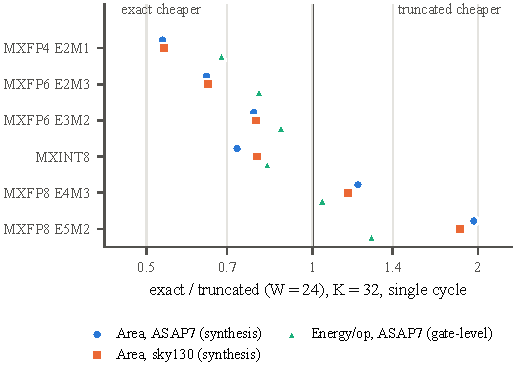
\includegraphics[width=\columnwidth]{figs/crossover.pdf}
\caption{Exact over truncating ($W=24$) unit, $K=32$, single cycle.  Below 1
the exact unit is cheaper.  Area agrees across both technologies; energy
follows area but with a smaller penalty for E5M2.}
\label{fig:cross}
\end{figure}

\begin{table}[t]
\centering
\caption{Exact / truncating ($W{=}24$) ratios, $K{=}32$, single cycle}
\label{tab:cost}
\setlength{\tabcolsep}{3.5pt}
\begin{tabular}{lrrrrrr}
\toprule
& \multicolumn{2}{c}{area (synth.)} & \multicolumn{2}{c}{ASAP7 after CTS} & \multicolumn{2}{c}{sky130 after CTS} \\
\cmidrule(lr){2-3}\cmidrule(lr){4-5}\cmidrule(lr){6-7}
Format & ASAP7 & sky130 & delay & energy & delay & energy \\
\midrule
E2M1 & 0.53 & 0.54 & 0.92 & 0.68 & 0.91 & 0.79 \\
E2M3 & 0.64 & 0.65 & 0.93 & 0.80 & --   & --   \\
E3M2 & 0.78 & 0.79 & 0.93 & 0.88 & --   & --   \\
INT8 & 0.73 & 0.79 & 1.15 & 0.83 & --   & --   \\
E4M3 & 1.21 & 1.16 & 1.01 & 1.04 & --   & --   \\
E5M2 & 1.96 & 1.85 & 1.10 & 1.28 & 1.11 & 1.19 \\
\bottomrule
\end{tabular}
\end{table}

Table~\ref{tab:cost} and Fig.~\ref{fig:cross} show the central result.  The
cost of exactness follows Table~\ref{tab:grid}: the exact unit's width
scales with each format's exponent range, whereas the truncating unit pays a
roughly fixed price for a $W$-bit window, $K$ alignment shifters and the
max-exponent tree.  For FP4, both FP6 formats and INT8 the exact unit is
21--47\% smaller and uses 12--32\% less energy.  It is also 7--9\% faster,
except for INT8, where it is 15\% slower.  E4M3 is near break-even:
+16--21\% area and +4\% energy against $W=24$, and within 5\% in area
against $W=32$, the width that nearly matches exact in the stress test.
Only E5M2, with a 69-bit grid, pays clearly: +85--96\% area.  Its energy
penalty is smaller, +19--28\%, because most of the wide grid rarely
switches.  Synthesis area ratios on the two technologies agree within 8\%
of each other for every format.

After CTS on sky130 the area ratios move towards 1 (FP4 0.65, E5M2 1.61).
The cause is placement-time design-rule repair, which on sky130 adds 7--25\%
area, unevenly between designs, plus fixed port buffers and tap cells; on
ASAP7 the same steps add 2--3\% and the post-CTS ratios match synthesis.
The direction of every result is unchanged.

\paragraph*{Block size}
The overhead of exactness is paid once per block (the wide final add and
normalisation), while alignment in the truncating unit is paid per element.
For pipelined E4M3 the area ratio falls from 1.31--1.34 at $K=8$ to
1.01--1.03 at $K=64$ on both technologies (Fig.~\ref{fig:k}).

\begin{figure}[t]
\centering
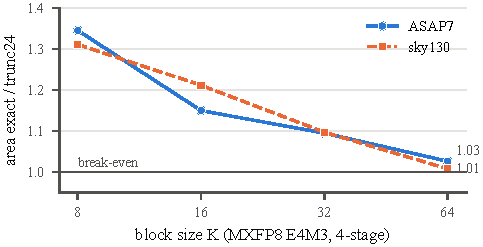
\includegraphics[width=\columnwidth]{figs/blocksize.pdf}
\caption{Area of exact over truncating ($W=24$) MXFP8 E4M3, 4-stage,
versus block size.  The per-block cost of exactness is amortised.}
\label{fig:k}
\end{figure}

\paragraph*{Pipelined units}
With the same four cut positions, the pipelined E4M3 exact unit reached
1.65\,ns against 2.67\,ns for the truncating unit after routing, with
+6\% area and +6\% energy.  Neither is stage-balanced (the truncating unit's
max-exponent search alone takes about 0.75\,ns), so we report these only as
indicative.

\section{Discussion}\label{sec:disc}
\paragraph*{Design rule}
For MXFP4, MXFP6 and MXINT8, exact accumulation is cheaper and more accurate
than a 24-bit truncating datapath and gives bit-reproducible,
order-independent results.  For MXINT8 it is also necessary for accuracy on
outlier data, at a 15\% delay cost.  For MXFP8 E4M3 exactness is roughly
free at $K=32$ and becomes free as $K$ grows.  Only MXFP8 E5M2 justifies
truncation on cost, and there $W=24$ is accurate in realistic accumulation.

\paragraph*{Limitations}
\begin{itemize}
  \item Error data is synthetic.  The outlier distribution approximates, but
        is not, real model tensors.
  \item Absolute delays from the open flow are pessimistic: much arithmetic
        maps to ripple full-adder chains (a 293-cell critical path even for
        a small FP4 configuration with $K=8$); only ratios on the same flow
        should be compared.
  \item Energy excludes glitch power, which may penalise the deeper design.
  \item The truncating baseline follows the standard organisation; published
        refinements such as anchor-based alignment~\cite{lutz2024fp8} or
        split global/local alignment~\cite{kaul2019dot} may shift its cost.
  \item Accumulation across blocks feeds $r$ back as $c$; an internal wider
        accumulator is not studied.
\end{itemize}

\section{Conclusion}
Whether an MX dot product should be exact depends on the format, and the
dependence is simple: exactness costs in proportion to the exponent range.
It is cheaper than truncation for four of the six formats, near free for
E4M3, and costly only for E5M2.  The RTL, bit-accurate models, verification
and flow scripts are available at
\ifdefined\ANON
\url{https://anonymous.4open.science/r/mx-dotp-arith}
\else
\url{https://github.com/allmahdyy/mx-dotp}
\fi
so that others can reproduce and extend these results.

% IEEE requires AI-generated content (text, figures, code) to be disclosed in
% the acknowledgments, naming the system and the parts it was used for.
% Check the wording against IEEE's current author guidelines and make sure
% it matches how the work was actually done.
\section*{Acknowledgment}
An AI assistant (Anthropic's Claude) was used throughout this work: to write
and debug the RTL, the Python reference and bit-true models, the cocotb
testbench and the synthesis, power and analysis scripts; to run the
experiments; to produce the figures; and to draft the text of this paper.
The author directed the study, reviewed the design, the verification
results and the method decisions, checked the reported numbers against the
raw data, and takes full responsibility for the content.

\bibliographystyle{IEEEtran}
\bibliography{refs}

\end{document}
